Современные интеллектуальные ассистенты являются многокомпонентными системами, организующими
среду взаимодействия, целевой сценарий диалога, персонализацию и приватность переписки. Конкретные компоненты
выбираются из целей и возможности команды разработчиков. Для исследовательских целей, как правило, используется
открытое программное обеспечение, требующее лишь незначительной адаптации под постановку. В этой секции 
будет описан подход к созданию цифрового ассистента для проведения исследования. 

Основой современных ассистентов является большая языковая модель,
обученная посредством техник оптимизации выполнять инструкции, описанные естественным языком. 
Модель прекрасно справляется с задачами коммуникации, придерживается делового этикета и демонстрирует эмпатические
внимание к проблемам пользователя \cite{jiang2023mistral} \cite{llamatouvron2023}.

Языковая модель также помогает в решении повседневных и деловых задач, сокращая академические статьи и помогая составлять
планы проектов. Последние достижения также позволяют задавать вопросы по изображениям, что существенно облегчает
выбор одежды и мебели \cite{bai2023qwen}. Тем не менее современные ассистенты не способны 
к выполнению формальных логические операции: арифметического сложения \cite{bubeck2023sparks}, решения абстрактных логических задач \cite{bordt2023chatgpt}, соблюдение 
правил стратегических игр \cite{Adam2024}.

\begin{figure}[h]
    \centering
    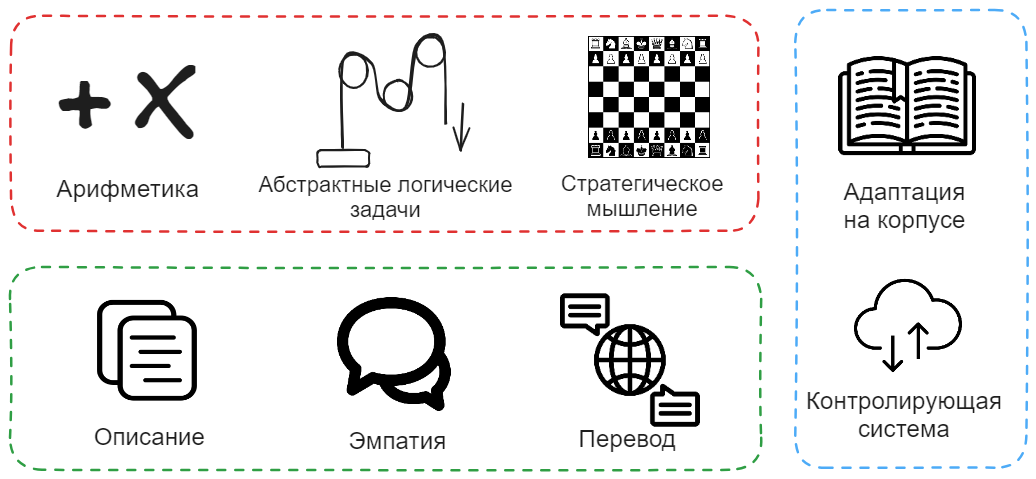
\includegraphics[width=0.5\textwidth]{assets/work/arch/problems.excalidraw.png}
    \caption{Навыки современного ассистента ограничены коммуникацией и решением базовых задач обработки текста}
    \label{problems}
\end{figure}

В образование интеллектуальные ассистенты применяются для обучения русском языку \cite{аль2019интеллектуальный} 
и рисования поясняющих графиков \cite{bulusuautomated}. Примерами коммерческого
использования ассистентов в образовании являются компании Merlin Mind
и OpenAI Education. Ключевым преимуществом решений является адаптация к общеобразовательным программ стран, 
взаимодействие с интерактивной доской и проприетарно подготовленная база знания регулярно обновляющая предметными экспертами.
